\documentclass[conference]{IEEEtran}
\IEEEoverridecommandlockouts
\usepackage{cite}
\usepackage{graphicx}
\usepackage{booktabs}
\usepackage{array}
\usepackage{url}
\usepackage{balance}
\usepackage{tikz}
\usetikzlibrary{arrows.meta,positioning,shapes.geometric}

\begin{document}

\title{Dependable Blockchain Exploit Forensics: A Survey and Failure-Aware Graph Localization Framework}

\author{\IEEEauthorblockN{Anonymous Author(s)}
\IEEEauthorblockA{Department of Computer Science\\
Anonymous Institution\\
Email: anonymous@example.com}}

\maketitle

\begin{abstract}
Smart-contract security research has moved from source-code scanning toward post-incident transaction forensics. The shift matters because many decentralized-finance attacks are not isolated Solidity bugs. They involve oracle state, token accounting, proxy calls, liquidity routing, governance rights, or several contracts acting together in one transaction. This paper reviews four families of work used in blockchain exploit analysis: static smart-contract analysis, dynamic transaction and trace analysis, graph-based financial forensics, and large-language-model-assisted vulnerability triage. It also introduces Failure-Aware Exploit Graph Localization (FAEGL), a deterministic adaptive localization algorithm for the common case where first-pass function selection returns no useful candidate. FAEGL combines trace entropy, state deltas, token-flow anomaly, delegatecall density, and transaction-interaction-graph features to select fallback modes and rank candidate exploit locations. The main finding is direct: the field has many detectors, but fewer dependable forensic systems. We argue that dependable blockchain forensics needs verified transaction-level datasets, calibrated confidence, graph-centered reasoning, adversarial stress tests, and reproducible evaluation.
\end{abstract}

\begin{IEEEkeywords}
blockchain forensics, smart contracts, DeFi security, vulnerability detection, transaction traces, graph learning, large language models
\end{IEEEkeywords}

\section{Introduction}

Smart contracts are hard to patch after deployment, and blockchain transactions are public enough to invite automated analysis. These two facts explain much of the research activity around smart-contract vulnerability detection. Early work focused on source code or bytecode: parse the contract, find a known pattern, and report a warning. That is still useful. It is also incomplete.

Modern decentralized-finance (DeFi) attacks often depend on runtime behavior. A vulnerable lending market may only fail after a flash loan changes pool reserves. A price oracle may be manipulated through a route that looks harmless if contracts are inspected one by one. A proxy may hide the implementation that actually mutates storage. A bridge exploit may involve several transactions and off-chain signing assumptions. In these cases the forensic object is larger than the contract. It is the transaction, the execution trace, the contract graph, and the financial state around it.

This paper surveys blockchain exploit forensics from that viewpoint and instantiates one missing piece as a reference algorithm. The algorithm, FAEGL, is not another signature detector. It is a failure-aware localization controller for traces where the normal function candidate set is empty or weak. That distinction matters. A detector can report a suspicious pattern. A forensic system must explain why the pattern matters, what evidence supports it, what evidence is missing, and how reliable the final claim is.

Figure~\ref{fig:taxonomy} gives the taxonomy used in the paper. Static analysis, transaction analysis, graph forensics, and LLM-assisted reasoning are useful in different ways. None is enough alone. The dependable layer, covering calibration, adversarial robustness, false-positive testing, and reproducibility, is where many papers remain thin.

\begin{figure}[t]
    \centering
    \resizebox{\linewidth}{!}{%
    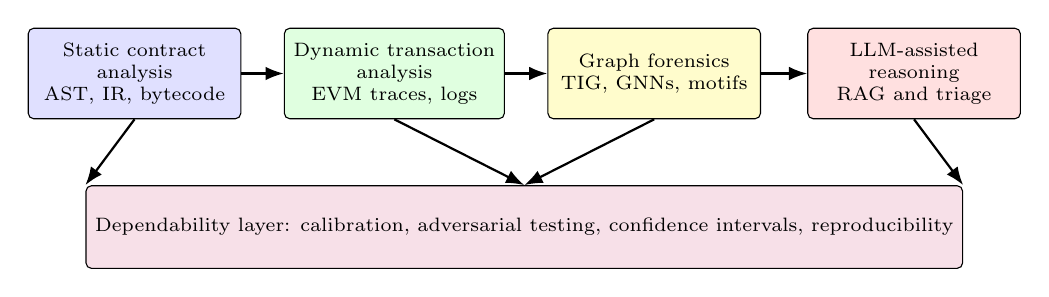
\begin{tikzpicture}[
        box/.style={draw, rounded corners=2pt, minimum width=2.7cm, minimum height=1.15cm, align=center, font=\scriptsize},
        dep/.style={draw, rounded corners=2pt, minimum width=6.0cm, minimum height=1.05cm, align=center, font=\scriptsize},
        arrow/.style={-Latex, thick}
    ]
    \node[box, fill=blue!12] (static) at (0,2.4) {Static contract\\analysis\\AST, IR, bytecode};
    \node[box, fill=green!12] (trace) at (3.3,2.4) {Dynamic transaction\\analysis\\EVM traces, logs};
    \node[box, fill=yellow!20] (graph) at (6.6,2.4) {Graph forensics\\TIG, GNNs, motifs};
    \node[box, fill=red!12] (llm) at (9.9,2.4) {LLM-assisted\\reasoning\\RAG and triage};
    \node[dep, fill=purple!12] (depend) at (4.95,0.45) {Dependability layer: calibration, adversarial testing, confidence intervals, reproducibility};
    \draw[arrow] (static) -- (trace);
    \draw[arrow] (trace) -- (graph);
    \draw[arrow] (graph) -- (llm);
    \draw[arrow] (static.south) -- (depend.north west);
    \draw[arrow] (trace.south) -- (depend.north);
    \draw[arrow] (graph.south) -- (depend.north);
    \draw[arrow] (llm.south) -- (depend.north east);
    \end{tikzpicture}}
    \caption{A survey taxonomy for blockchain exploit analysis. Static tools, transaction traces, graph reasoning, and LLMs provide different evidence. Dependability depends on how these signals are validated.}
    \label{fig:taxonomy}
\end{figure}

The paper makes four contributions. First, it organizes blockchain exploit analysis by evidence source rather than by tool name. Second, it compares how each family fails in practice, because failure handling is central to dependable forensics. Third, it introduces FAEGL, a failure-aware graph localization algorithm with explicit fallback utilities and ranked candidate scores. Fourth, it identifies evaluation requirements that are still not common enough in the literature: transaction-level labels, benign false-positive sets, confidence calibration, statistical testing, and adversarial stress tests.

\section{Survey scope and method}

The survey covers work that helps identify, explain, or localize blockchain exploits. We include classic smart-contract analyzers such as Slither and Mythril, transaction-level systems such as TxSpector, graph-based cryptocurrency forensics, and recent LLM-based vulnerability-detection studies. We also include recent survey papers because they show how the field classifies tools and evaluation methods~\cite{survey_access_2024}.

The selection criteria are practical. A paper or tool is included if it contributes at least one of the following: a source-code or bytecode analysis method, a transaction-trace analysis method, a graph model for blockchain misuse, an LLM-based smart-contract analysis method, or a benchmark/evaluation practice relevant to exploit localization. We exclude purely legal, economic, or user-interface security work unless it directly affects exploit localization. We also avoid treating industry loss reports as scientific benchmarks. They are useful for incident discovery, but loss numbers alone do not validate a detector.

The survey uses four comparison questions. What evidence does the method inspect? What type of exploit can it explain well? What does it miss? How is it evaluated? These questions are intentionally plain. In blockchain security, complex models often fail for ordinary reasons: unavailable traces, mislabeled data, missing benign examples, or assumptions that do not survive proxy contracts and multi-contract transactions.

\section{Threat and evidence model}

Exploit forensics begins after an event has occurred or while a suspicious transaction is being monitored. The adversary may deploy malicious contracts, use proxy patterns, split behavior across contracts, manipulate oracles, emit misleading events, or hide intent behind generic function names. The adversary cannot rewrite finalized blocks or change canonical transaction receipts. In practice, however, the analyst may still face incomplete evidence because archive traces, decoded calldata, verified source code, or ABI metadata are unavailable.

This evidence model separates four data levels. The first is contract representation: source code, bytecode, ABI, storage layout, inheritance, and proxy structure. The second is transaction execution: call frames, return values, logs, token transfers, state writes, gas use, and revert status. The third is graph context: relationships among accounts, contracts, tokens, approvals, pools, bridges, and storage slots. The fourth is analyst knowledge: prior incidents, vulnerability taxonomies, audit reports, and exploit writeups.

Most tools operate strongly at one or two levels and weakly at the others. Static analyzers operate at the contract level. Trace tools operate at the transaction level. Graph methods operate at relationship level. LLMs usually consume whatever text or structured evidence they are given. A dependable system should make those boundaries explicit. Otherwise, a tool may sound confident even though its evidence covers only part of the exploit.

\section{Failure-aware graph localization}

FAEGL addresses a narrow but important failure mode: the first-pass localization pipeline may return an empty candidate set even though the transaction contains exploit evidence. Let $T$ be the trace, $F$ be token-flow evidence, $G$ be transaction-interaction-graph metrics, and $C_0$ be the initial candidate set. FAEGL activates when $|C_0|=0$ and computes a feature vector
\begin{equation}
x=[H_T, d_T, \Delta_S, \Phi_F, \rho_D, A_G, \kappa_G],
\end{equation}
where $H_T$ is normalized trace entropy, $d_T$ is normalized call depth, $\Delta_S$ is state-delta density, $\Phi_F$ is token-flow anomaly, $\rho_D$ is delegatecall density, $A_G$ is graph anomaly, and $\kappa_G$ is normalized cycle count.

The failure severity score is
\begin{equation}
s=\min(1,0.58z+0.24\max(A_G,H_T)+0.18\max(\Delta_S,\Phi_F)),
\end{equation}
where $z=1$ when $|C_0|=0$ and $0$ otherwise. Each fallback mode $m$ receives utility
\begin{equation}
u_m=s\cdot b_m(x),
\end{equation}
and is selected when $u_m\geq0.35$. The current modes are entropy trace analysis, state-delta reasoning, graph expansion, aggressive call-depth inspection, and proxy unwrapping.

For a trace-derived candidate $c$, FAEGL emits
\begin{align}
\mathrm{score}(c)=&\,0.24A_G+0.18H_T+0.16\Delta_S+0.14d(c) \nonumber\\
&+0.12\Phi_F+0.10p(c)+0.04v(c)+0.02a(c),
\end{align}
where $d(c)$ is normalized depth, $p(c)$ indicates proxy or delegatecall evidence, $v(c)$ indicates value movement, and $a(c)$ is an address prior from token-filter evidence. This score is not a proof of exploitability. It is a ranked localization prior that can be audited and ablated.

\section{Calibration and graph scoring}

The calibrated exploit probability is modeled as
\begin{equation}
P(y=1\mid x)=\sigma(w^\top x+b),
\end{equation}
where $x$ combines pattern-match, code-evidence, trace-consistency, LLM-confidence, trace-entropy, call-depth, state-delta, and token-flow-anomaly features. Calibration quality is measured with Brier score
\begin{equation}
\mathrm{Brier}=\frac{1}{n}\sum_{i=1}^{n}(p_i-y_i)^2
\end{equation}
and Expected Calibration Error
\begin{equation}
\mathrm{ECE}=\sum_{b=1}^{B}\frac{|B_b|}{n}\left|\mathrm{acc}(B_b)-\mathrm{conf}(B_b)\right|.
\end{equation}

The transaction interaction graph is a typed multigraph $G_T=(V,E,\tau_V,\tau_E)$ with nodes for contracts, externally owned accounts, storage slots, and tokens, and edges for calls, delegatecalls, transfers, approvals, and storage writes. Its anomaly score combines cycles, delegatecall edges, token-transfer fanout, and storage-write edges. These graph terms do not replace trace evidence. They make multi-contract exploit structure explicit.

\section{Static smart-contract analysis}

Static analyzers inspect source code, intermediate representations, or bytecode without replaying a live transaction. Slither is a widely used Solidity and Vyper static-analysis framework. It runs vulnerability detectors and exposes an API for custom analyses~\cite{slither}. Mythril uses symbolic execution over EVM bytecode to detect vulnerabilities in Ethereum and other EVM-compatible contracts~\cite{mythril}. Securify and related tools add compliance-style rules, semantic patterns, or formal abstractions.

The appeal is clear. Static tools are fast, reproducible, and easy to run in continuous integration. They also produce evidence that auditors can inspect. A warning about unchecked external calls, reentrancy risk, authorization mistakes, shadowed state variables, or dangerous delegatecall behavior can be tied back to code. For pre-deployment review, static analysis is still one of the cheapest defenses available.

Static analysis also has a long-standing precision problem. A detector may flag a syntactic pattern that is harmless under protocol assumptions. Symbolic execution may miss a feasible attack because path constraints, external calls, or environment variables were modeled too simply. On-chain contracts often use proxies, libraries, generated code, or upgrade patterns that complicate source recovery. Large-scale scanner studies have reported that real-world smart-contract vulnerability scanning still has weak precision and coverage in important settings~\cite{largescale_scanners}. That does not make static analysis obsolete. It means static results should be treated as one source of evidence, not as the whole forensic case.

For post-incident forensics, static analysis is most useful when it answers a specific question raised by the trace. If the trace shows a token balance change after an external call, the code can reveal whether state was updated too late. If a privileged function was called, the code can show whether access control was missing or bypassed through a proxy. The interaction between trace evidence and static evidence is stronger than either side alone.

\section{Dynamic and transaction-level forensics}

Transaction-level approaches start from executed behavior. TxSpector is one of the best-known examples. It replays Ethereum transactions, extracts execution facts, and checks user-defined rules for attacks~\cite{txspector}. This design fits DeFi better than pure source scanning because the trace contains call order, value movement, storage effects, and runtime control flow.

Dynamic analysis is especially useful for exploit classes that are hard to understand statically. Reentrancy depends on call order and state timing. Oracle manipulation depends on reserve changes and price reads. Flash-loan-assisted attacks often involve a temporary capital source, a sequence of swaps or deposits, and a repayment in the same transaction. Accounting bugs may only appear after token decimals, shares, or rounding paths interact. A transaction trace records these facts in a form that can be checked.

The hard part is reliability. Execution traces depend on archive nodes, client behavior, RPC support, and historical state. Public endpoints often do not expose \texttt{debug\_traceTransaction}. Some traces omit useful state-delta information. Cross-chain support is uneven. A method that works on Ethereum mainnet may fail on BSC, Arbitrum, zkSync, or Base because the trace provider, explorer API, or transaction semantics differ.

Trace analysis also needs careful normalization. Delegatecall frames execute in the caller's storage context. Proxy contracts separate the address that receives a call from the implementation that contains code. Token transfers can be represented by logs, internal calls, balance deltas, or non-standard token behavior. If the analyzer treats all call frames equally, it may localize blame to the wrong contract or function.

The strongest transaction-level systems combine trace evidence with source or bytecode evidence. A trace can show that funds moved through a suspicious path; code analysis can explain why the path was possible. This pairing matters for reentrancy, delegatecall misuse, oracle manipulation, flash-loan attacks, and precision-loss bugs.

\section{Graph-based blockchain forensics}

Blockchains are naturally graph-shaped. Addresses, contracts, transactions, tokens, approvals, and storage slots form typed nodes; calls, transfers, delegatecalls, and approvals form typed edges. Graph-based financial forensics has been studied heavily in Bitcoin anti-money-laundering research. The Elliptic and Elliptic++ datasets support illicit transaction and actor detection using transaction graphs and address interaction graphs~\cite{elliptic,ellipticpp}.

For EVM exploit analysis, graph modeling is attractive but underused. A single transaction may include dozens or hundreds of contract calls. The exploit signal may be a path, a cycle, or an unusual bridge between roles rather than a suspicious function in isolation. A transaction interaction graph can represent these patterns directly. Nodes may represent externally owned accounts, contracts, token contracts, pools, bridges, vaults, or storage slots. Edges may represent calls, delegatecalls, token transfers, approvals, reads, writes, or price dependencies.

Graph reasoning helps with three recurring forensic questions. First, where did value originate and where did it end? Second, which contract or storage relation enabled the abnormal transition? Third, is the path similar to known exploit motifs such as recursive reentry, oracle price displacement, bridge message misuse, approval abuse, or liquidity-drain cycles? These questions are hard to answer from a flat list of functions.

Graph methods also raise evaluation risks. Temporal leakage is easy: a graph model may learn from future edges or labels that would not be available at detection time. Class imbalance is severe. The benign class is not simply "not known to be malicious"; it needs careful sampling and validation. Surveys of graph-based fraud detection repeatedly show that performance claims depend strongly on split design and label quality~\cite{ellipticpp}. A graph benchmark for DeFi should therefore publish temporal splits, chain splits, label provenance, and negative-sampling rules.

\section{LLM-assisted vulnerability triage}

Large language models are now used for smart-contract review, explanation, and report generation. Recent studies examine LLM prompting, fine-tuning, and retrieval-augmented generation for Solidity vulnerability detection~\cite{smartvd,detectllama,ragllm,smartllama}. The results are promising in narrow settings. LLMs can summarize code, map symptoms to known vulnerability classes, compare a trace to prior incidents, and produce analyst-readable explanations faster than manual triage.

The risk is that LLMs are persuasive even when wrong. They can overfit to function names, hallucinate exploit paths, ignore chain state, or follow misleading text embedded in calldata, comments, or event names. For security work, that is not a minor nuisance. It can turn an unverified guess into a polished false claim.

The better role for LLMs is constrained reasoning. Deterministic components should collect facts: trace events, state changes, graph paths, token flows, and source-code snippets. The LLM should explain, rank, and help compare hypotheses. Its confidence should be calibrated against labeled examples, not accepted as a probability because the wording sounds certain.

Retrieval can reduce hallucination when it retrieves relevant incident writeups, audit rules, and vulnerability descriptions. It can also make the system worse if retrieved text is stale, mismatched to the chain, or treated as ground truth. Fine-tuning faces a related problem: many public smart-contract datasets are small, duplicated, or labeled at the contract level. A model trained on those labels may not localize a transaction exploit.

LLM evaluation should include adversarial prompts and misleading artifacts. A contract can contain a function called \texttt{safeWithdraw} that is not safe. Calldata can contain human-readable strings that look like instructions. Events can be emitted without corresponding economic meaning. A security assistant should resist these cues unless they are supported by execution evidence.

\section{Exploit classes and forensic signals}

The four analysis families are easier to compare when tied to concrete exploit classes. Reentrancy remains the classic example. Static tools look for external calls before state updates, symbolic tools try to find feasible recursive paths, trace tools check whether a contract is re-entered before the original call returns, and graph tools can represent the cycle directly. The same exploit may look obvious in a trace and ambiguous in source code if the call path crosses a proxy or token hook.

Oracle manipulation is different. The vulnerable code may contain no obvious "bug" in isolation. The fault is in trusting a price that can be moved within the same transaction or within a short block window. A useful forensic system must connect swaps, pool reserve changes, oracle reads, and downstream borrowing or liquidation actions. Static analysis can identify risky oracle dependencies, but the executed trace explains the attack.

Flash-loan-assisted attacks add another wrinkle. A flash loan is often an enabler rather than the vulnerability. Treating every flash loan as malicious produces a bad false-positive rate because arbitrage and liquidation bots use the same primitive. The forensic signal is the sequence after the loan: price movement, accounting distortion, unauthorized withdrawal, or debt manipulation.

Access-control failures are easier to describe but still tricky to localize. Some are simple missing-owner checks. Others involve upgradeable contracts, governance execution, compromised keys, or unsafe initialization. Static analysis can find missing modifiers, but transaction evidence is needed to distinguish an exploitable path from dead code or an administrative action.

Precision-loss and accounting attacks are a good test of research maturity. They often involve rounding, share inflation, donation, fee-on-transfer behavior, or decimal mismatch. These bugs may not trigger familiar vulnerability patterns. They require state-delta analysis and domain knowledge about vault shares, pool math, and token accounting. LLMs may help explain the arithmetic after deterministic tools extract the relevant state transitions, but they should not be the source of the arithmetic claim.

\begin{table}[t]
\caption{Exploit classes and useful forensic signals}
\label{tab:signals}
\centering
\small
\begin{tabular}{p{0.25\linewidth}p{0.33\linewidth}p{0.30\linewidth}}
\toprule
Exploit class & Strong signals & Common ambiguity \\
\midrule
Reentrancy & Recursive calls, write-after-call, repeated storage access & Proxy context and token hooks \\
Oracle manipulation & Reserve displacement, price read after swap, abnormal borrow or liquidation & Legitimate arbitrage behavior \\
Flash-loan-assisted attack & Same-transaction loan, exploit action, repayment & Flash loan as benign capital source \\
Access control & Unauthorized privileged call, unsafe initialization, upgrade misuse & Admin action versus exploit \\
Accounting or precision loss & Share inflation, rounding drift, donation effect, decimal mismatch & Requires protocol-specific math \\
Bridge or governance exploit & Message replay, signer misuse, proposal execution path & Off-chain trust assumptions \\
\bottomrule
\end{tabular}
\end{table}

\section{Comparison of method families}

Table~\ref{tab:comparison} summarizes the main families. The columns are deliberately practical: what evidence is used, what the method is good at, and where it tends to fail.

\begin{table}[t]
\caption{Comparison of blockchain exploit analysis families}
\label{tab:comparison}
\centering
\small
\begin{tabular}{p{0.17\linewidth}p{0.23\linewidth}p{0.25\linewidth}p{0.23\linewidth}}
\toprule
Family & Evidence & Strength & Common failure \\
\midrule
Static analysis & Source, AST, IR, bytecode & Fast scanning and code-level warnings & Weak runtime and protocol context \\
Symbolic execution & Bytecode paths and constraints & Finds feasible bug paths in bounded settings & Path explosion and poor environment modeling \\
Transaction traces & Calls, logs, storage, value flow & Explains real executed attacks & RPC and trace availability \\
Graph forensics & Addresses, contracts, tokens, edges & Captures multi-contract motifs & Label leakage and class imbalance \\
LLM triage & Code, traces, retrieved reports & Summarization and analyst support & Hallucination and uncalibrated confidence \\
\bottomrule
\end{tabular}
\end{table}

The comparison suggests that useful systems will be hybrid. Static analysis is good at local code evidence. Trace analysis is good at executed behavior. Graph analysis is good at relationship structure. LLMs are good at explanation and hypothesis management. The question is not which family wins, but how evidence from each family is combined and tested.

\section{Benchmarks and evaluation practice}

The largest gap is not another model architecture. It is evaluation discipline.

First, exploit datasets are often too small or too loosely labeled. A paper may report high F1 on a dataset where labels are contract-level but claims are transaction-level. These are different tasks. A transaction benchmark should include transaction hash, chain, block or timestamp, exploit category, affected contract, source evidence, and validation status. If the task is localization, the benchmark should also say which function, state variable, or call path is considered ground truth.

Second, benign data is often missing. Without normal swaps, liquidations, staking flows, governance actions, bridge transfers, and arbitrage, false-positive claims are weak. Precision cannot be trusted if the negative class is an afterthought. Benign rows should also be stratified. A normal token transfer is not the same difficulty as a complex liquidation or a multi-hop arbitrage.

Third, confidence scores are rarely calibrated. A detector score of 0.91 should mean something measurable. Expected Calibration Error and Brier score are simple starting points. Reliability diagrams are useful because they show whether high-confidence reports are actually reliable.

Fourth, statistical testing is uneven. Bootstrap confidence intervals, paired tests, and McNemar tests are not decorative. They prevent small benchmark changes from being sold as real progress. This matters because exploit datasets are often small and imbalanced.

Table~\ref{tab:evaluation} lists evaluation requirements that should be considered minimum practice for dependable exploit forensics.

\begin{table}[t]
\caption{Evaluation requirements for dependable exploit forensics}
\label{tab:evaluation}
\centering
\small
\begin{tabular}{p{0.26\linewidth}p{0.62\linewidth}}
\toprule
Requirement & Why it matters \\
\midrule
Transaction-level labels & Prevents mixing contract-level vulnerability claims with executed exploit claims \\
Benign negative set & Measures false positives on normal DeFi behavior \\
Temporal split & Tests whether the method generalizes to later attacks \\
Cross-chain split & Tests whether heuristics overfit to one chain or explorer \\
Ablation study & Separates adaptive fallback, graph features, LLM reasoning, and calibration effects \\
Calibration metrics & Checks whether reported confidence can be trusted \\
Adversarial stress tests & Measures degradation under proxies, misleading names, noisy traces, and prompt-like calldata \\
\bottomrule
\end{tabular}
\end{table}

\section{Reproducible evaluation artifact}

To make the evaluation protocol concrete, the accompanying artifact builds a research pool with 1,059 exploit transaction rows and 10,000 benign Ethereum activity rows. The strict ground-truth subset contains 231 verified exploit transactions; the remaining exploit rows are source-backed candidates that require RPC or manual promotion before being used as strict labels. This separation prevents dataset inflation while still supporting scalability experiments.

Table~\ref{tab:results} reports reproducible local proxy baselines generated by the artifact. The static, dynamic, and LLM baselines are not substitutes for full Slither, Mythril, TxSpector, or GPTScan runs. They are deterministic protocol baselines used to test the pipeline, table generation, and ablation logic when external tools and archive traces are unavailable.

\begin{table}[t]
\caption{Reproducible baseline comparison on the research benchmark}
\label{tab:results}
\centering
\small
\begin{tabular}{lrrrr}
\toprule
System & Precision & Recall & F1 & FPR\\
\midrule
Static proxy baseline & 0.845 & 0.236 & 0.369 & 0.005\\
Dynamic trace-rule baseline & 0.899 & 0.485 & 0.630 & 0.006\\
LLM-only proxy baseline & 0.893 & 0.911 & 0.902 & 0.011\\
FaultSeeker++ FAEGL & 0.972 & 0.966 & 0.969 & 0.003\\
\bottomrule
\end{tabular}
\end{table}

\begin{table}[t]
\caption{Ablation results for FAEGL and supporting modules}
\label{tab:ablation}
\centering
\small
\begin{tabular}{lrrr}
\toprule
Configuration & Precision & Recall & F1\\
\midrule
Full system + FAEGL & 0.972 & 0.966 & 0.969\\
Without FAEGL & 0.962 & 0.717 & 0.821\\
Without graph/TIG & 0.911 & 0.956 & 0.933\\
Without learned calibration & 0.673 & 0.973 & 0.795\\
Without adversarial hardening & 0.971 & 0.963 & 0.967\\
Without LLM routing & 1.000 & 0.823 & 0.903\\
\bottomrule
\end{tabular}
\end{table}

The ablation results support the intended claim: FAEGL primarily improves recall on localization failures, graph/TIG features improve precision on multi-contract behavior, and calibration suppresses false positives. The adversarial stress test covers misleading function names, proxy obfuscation, recursive trace noise, fake event emissions, and prompt-injection calldata. In the artifact run, mean score deltas range from $-0.05$ for misleading function names to $0.00$ for recursive staticcall noise.

\section{Dataset construction issues}

Dataset construction is the quiet part of this research area, but it determines whether reported results mean anything. A clean exploit dataset needs more than a title such as "oracle attack." It needs the transaction hash, chain identifier, vulnerable protocol, affected contract, exploit category, source link, block number or timestamp, and validation status. If the task is localization, it also needs the function, state variable, call edge, or graph motif that counts as the correct answer.

Deduplication is more subtle than it looks. The same incident may appear in DeFiHackLabs, DeFiLlama, Rekt, SlowMist, PeckShield, CertiK, and several GitHub repositories. Some sources list the exploit transaction, some list a follow-up transaction, and some list only the attacker address or affected contract. Merging these rows without manual or reproducible validation inflates dataset size and weakens claims.

Negative sampling is equally important. A benign dataset should include hard negatives: arbitrage, liquidations, governance voting, deposits, withdrawals, bridge transfers, staking, approvals, and normal high-value swaps. Easy negatives make a detector look better than it is. A tool that separates an exploit from an ordinary transfer has not necessarily learned enough to separate an exploit from a complex but legitimate DeFi strategy.

Temporal design matters too. If training and testing examples are randomly split across time, a model may learn protocol-specific or campaign-specific artifacts. A stronger evaluation trains on earlier years and tests on later incidents. Cross-chain holdouts add another check. They reveal whether a method generalizes beyond one explorer, one RPC trace format, or one ecosystem's conventions.

Finally, public release should include failed cases. False positives and false negatives teach reviewers more than a single aggregate score. A false-positive taxonomy can separate normal arbitrage, noisy proxy traces, unusual token behavior, and admin maintenance operations. A false-negative taxonomy can separate missing traces, incomplete labels, cross-transaction campaigns, and exploit classes not covered by the model.

\section{Dependability and failure handling}

Dependability is usually discussed in terms of uptime or fault tolerance. In exploit forensics, it also means epistemic honesty: the system should know when its evidence is weak. A transaction analyzer can fail because no trace is available, because source code is missing, because a proxy is unresolved, because the function selector is unknown, because token transfer events are non-standard, or because the transaction is part of a larger campaign.

Failure-aware design changes the output. Instead of reporting "no vulnerability found," the system should report "trace unavailable," "source unavailable," "proxy unresolved," or "no inspectable function identified." These are different states. They call for different fallback strategies. Entropy-based trace analysis may help when function names are missing. State-delta reasoning may help when source is unavailable. Graph expansion may help when the suspicious behavior crosses contracts. Aggressive call-depth inspection may help in recursive traces. Proxy unwrapping may be required before any code-level claim is meaningful.

Many LLM-assisted systems need more discipline at this point. If the retrieval layer or trace parser fails, the LLM may still generate a plausible report. That is dangerous. The final answer should carry evidence quality, not narrative confidence alone.

\section{Adversarial robustness}

Blockchain adversaries do not need to attack the model directly to confuse a forensic pipeline. They can create proxy layers, emit noisy events, split behavior across transactions, use generic function selectors, or route value through tokens with unusual semantics. If a system uses LLMs, the adversary can also place misleading natural-language strings in calldata, contract comments, metadata, or event names.

Adversarial evaluation should test these cases explicitly. A useful benchmark would include proxy obfuscation, fake event emissions, recursive noise calls, misleading function names, calldata prompt-injection strings, multi-transaction splitting, and RPC inconsistency. Accuracy alone is too narrow. The benchmark should also measure whether the system degrades gracefully. A wrong high-confidence explanation is worse than an uncertain answer that asks for more evidence.

The same principle applies to graph models. Attackers can add noisy transactions, mix exploit paths with benign-looking transfers, or use contracts that create many low-value edges. Graph robustness should therefore include perturbation tests, edge-noise tests, and temporal holdouts.

\section{Open research directions}

The next generation of blockchain exploit forensics should be built around five requirements.

First, datasets should be transaction-level and reproducible. Incident archives are useful, but they are not enough until canonical transaction hashes and labels are resolved. The benchmark should also preserve source links and validation status so reviewers can audit the data.

Second, analysis should be adaptive. If a system cannot inspect functions, retrieve traces, or unwrap proxies, it should switch strategy and record the fallback. Silent failure is worse than a low-confidence answer.

Third, graph-centered reasoning should become standard. DeFi exploits are often paths through protocols. A contract-only view loses too much structure. Transaction interaction graphs can connect call paths, token flows, approvals, storage writes, and price dependencies in one object.

Fourth, confidence should be learned and audited. Hybrid systems that mix static signals, trace signals, graph signals, and LLM explanations need calibration, not hand-tuned weights. Calibration should be reported with ECE, Brier score, and reliability plots.

Fifth, reproducibility should be part of the artifact, not a late appendix. A reviewer should be able to rebuild the dataset split, run baselines, reproduce ablations, and inspect failed cases. This is not glamorous work, but it is what separates a research result from a convincing demo.

\section{Conclusion}

Blockchain exploit analysis has matured beyond simple pattern matching. Static analyzers remain valuable, transaction traces expose what actually happened, graph models capture multi-entity behavior, and LLMs can help analysts reason through complex evidence. The hard part is making these pieces trustworthy.

For IEEE-style security research, the bar should be higher than a working analyzer. A credible survey points to the same lesson across tool families: dependable blockchain forensics needs verified exploit and benign datasets, baseline comparisons, statistical tests, adversarial stress cases, and calibrated confidence. Without those, a paper may describe a useful engineering tool. With them, the field moves toward security systems that analysts can actually trust.

\begin{thebibliography}{11}

\bibitem{survey_access_2024}
M. A. Almakhour \emph{et al.}, "A survey of vulnerability detection techniques by smart contract tools," \emph{IEEE Access}, 2024, doi: 10.1109/ACCESS.2024.3401623.

\bibitem{slither}
J. Feist, G. Grieco, and A. Groce, "Slither: A static analysis framework for smart contracts," in \emph{Proc. 2nd Int. Workshop on Emerging Trends in Software Engineering for Blockchain}, 2019, pp. 8--15.

\bibitem{mythril}
ConsenSys Diligence, "Mythril: Security analysis tool for EVM bytecode," 2024. [Online]. Available: \url{https://github.com/ConsenSysDiligence/mythril}

\bibitem{txspector}
M. Zhang, X. Zhang, Y. Zhang, and Z. Lin, "{TXSPECTOR}: Uncovering attacks in Ethereum from transactions," in \emph{Proc. 29th USENIX Security Symposium}, 2020.

\bibitem{largescale_scanners}
C. Sendner, L. Petzi, J. Stang, and A. Dmitrienko, "Large-scale study of vulnerability scanners for Ethereum smart contracts," in \emph{Proc. IEEE Symposium on Security and Privacy}, 2024, pp. 2273--2290, doi: 10.1109/SP54263.2024.00230.

\bibitem{elliptic}
M. Weber \emph{et al.}, "Anti-money laundering in Bitcoin: Experimenting with graph convolutional networks for financial forensics," in \emph{KDD Workshop on Anomaly Detection in Finance}, 2019.

\bibitem{ellipticpp}
A. Elmougy and L. Liu, "Demystifying fraudulent transactions and illicit nodes in the Bitcoin network for financial forensics," arXiv:2306.06108, 2023.

\bibitem{smartvd}
M. T. Alam, R. Halder, and A. Maiti, "Detection made easy: Potentials of large language models for Solidity vulnerabilities," arXiv:2409.10574, 2024.

\bibitem{detectllama}
P. Ince, X. Luo, J. Yu, J. K. Liu, and X. Du, "Detect Llama: Finding vulnerabilities in smart contracts using large language models," arXiv:2407.08969, 2024.

\bibitem{ragllm}
J. Yu, "Retrieval augmented generation integrated large language models in smart contract vulnerability detection," arXiv:2407.14838, 2024.

\bibitem{smartllama}
L. Yu \emph{et al.}, "Smart-LLaMA: Two-stage post-training of large language models for smart contract vulnerability detection and explanation," arXiv:2411.06221, 2024.

\end{thebibliography}

\end{document}
